\chapter{The optimal setup}\label{cha:the-optimal-setup}


\begin{figure}[!htbp]
  \centering
  \def\svgwidth{0.9\textwidth}
  \input{./../figures/problem-geometry.pdf_tex}
  \caption{My problem}
\end{figure}


\section{Orientation}
$E_N$ depending on the orientation:

\begin{equation}
  E_N = \log_2\left\{
    1 + \abs{
      \sin(
      \frac{G M_A M_B t}{\hbar} \frac{\Delta x_A \Delta x_B}{8L^3}
      \left[ \sin\alpha\sin\beta - \frac{1}{2}\cos\alpha\cos\beta \right]
      )
      }
  \right\}
\end{equation}

Time till the maximum entanglement ($E_N = 1$):
\begin{equation}
  t_\mathrm{max} = \frac{8 \pi L^3 \hbar}{2 G M_A M_B \Delta x_A\Delta x_B} \abs{\sin\alpha\sin\beta - \frac{1}{2}\cos\alpha\cos\beta}^{-1}
\end{equation}

with a global minimum for $\alpha,\beta \in [0, \pi]$ for the orthogonal orientation with $\alpha = \beta = \pi/2$. Here, the time till the maximum entanglement is given by
\begin{equation}
  t_\mathrm{max} = \frac{4 \pi \hbar L^3}{G M_A M_B \Delta x_A \Delta x_B} \simeq 129\si{mn}
\end{equation}

\begin{figure}[!htbp]
  \centering
  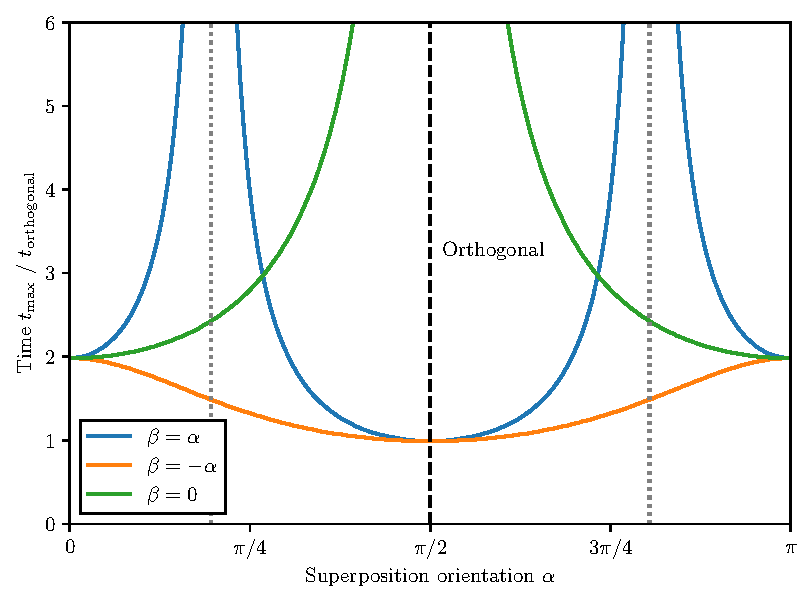
\includegraphics[width=\textwidth]{./../figures/EN-orientation.pdf}
  \caption{...}
  \label{fig:5:optimal-orientation}
\end{figure}



